We run the production formula agent with two local models, \efAName{} and \efBName, and three hosted ones, \efDName, \efEName{} and \efFName{} (Section~\ref{sec:e5method}). With the final system the first attempt is correct for \efAfinal\% of the \efAN{} tasks with \efAName{} and \efBfinal\% with \efBName; the hosted models reach \efDfinal\% (\efDN{} tasks), \efEfinal\% (\efEN) and \efFfinal\% (\efFN).

\paragraph{Retrieved context needs column letters}
\begin{table}
\caption{Attempt-1 execution accuracy (\%) by context. Lookup tasks read a sheet other than the active one; ``Other'' tasks read the active sheet only. The only difference between the two retrieved rows is that table chunks now carry column letters and the data-row span.}
\label{tab:e5-context}

\centering\footnotesize
\begin{adjustbox}{max width=\columnwidth}\begin{tabular}{l l rrr}
\toprule
\textbf{Model} & \textbf{Context} & \textbf{All} & \textbf{Lookup} & \textbf{Other} \\
\midrule
\multirow{3}{*}{Llama~3.1 8B} & Active sheet only & 72.2 & 3.3 & 78.5 \\
 & Retrieved (shipped) & 64.4 & 0.0 & 70.3 \\
 & Retrieved + letters & \textbf{70.8} & 0.0 & 77.3 \\
\midrule
\multirow{2}{*}{Llama~3.2 3B} & Active sheet only & 37.5 & 3.3 & 40.6 \\
 & Retrieved + letters & \textbf{38.9} & 3.3 & 42.1 \\
\midrule
\multirow{2}{*}{Llama~3.1 8B, new tasks} & Active sheet only & 76.7 & 0.0 & 80.7 \\
 & Retrieved + letters & \textbf{72.2} & 0.0 & 76.0 \\
\midrule
\multirow{2}{*}{Gemini~3.1 Flash-Lite} & Active sheet only & 89.2 & 31.8 & 95.0 \\
 & Retrieved + letters & \textbf{96.7} & 95.5 & 96.8 \\
\midrule
\multirow{2}{*}{Gemini~3.5 Flash-Lite} & Active sheet only & 89.9 & 27.3 & 96.0 \\
 & Retrieved + letters & \textbf{95.2} & 95.5 & 95.1 \\
\midrule
\multirow{2}{*}{Gemma~4 26B-A4B} & Active sheet only & 91.1 & 36.7 & 96.1 \\
 & Retrieved + letters & \textbf{95.8} & 96.7 & 95.8 \\
\bottomrule
\end{tabular}\end{adjustbox}
\end{table}

With the shipped active-sheet context \efAName{} reaches \efAflat\% at attempt 1 (Table~\ref{tab:e5-context}). Adding the ranked context in the chunk format the add-on shipped \emph{lowered} accuracy to \efAshipped\% (\efATestshippedvsflatB{} tasks favour the active sheet alone, \efATestshippedvsflatA{} the retrieved context; $p$ \efATestshippedvsflatP, exact McNemar). Those chunks listed columns by header only, so the model guessed letters (a silently wrong numeric column), wrote headers as names (\code{COUNTIF(Lead Time,">31")}) or invented functions. With each column's letter and the data-row span in the chunk, accuracy is \efAfinal\% ($p$ \efATestfinalvsshippedP{} against the shipped format), indistinguishable from the active sheet alone ($p$ \efATestfinalvsflatP): retrieval does not help on tasks that read the active sheet; its purpose is cross-sheet requests. There the first attempt is correct \efAfinalLookup\% of the time on the \efAfinalLookupN{} lookup tasks, because of the prompt rather than the context: \efALkSheetTwo{} of \efALkN{} attempts copied \code{Sheet2} from the agent's own worked example (Section~\ref{sec:discussion}). For the hosted models the retrieved context is what matters: it raises accuracy from \efDflat\%, \efEflat\% and \efFflat\% with the active sheet alone to \efDfinal\%, \efEfinal\% and \efFfinal\%, almost entirely on cross-sheet lookups (\efDflatLookup\% to \efDfinalLookup\% for \efDName).
\ifdefined\efCN
\emph{Held-out confirmation.} On \efCN{} tasks from fresh workbooks the final chunk format gives \efCfinal\% at attempt 1 against \efCflat\% for the active sheet alone ($p$ \efCTestfinalvsflatP), the same picture as on the main set. \gc{} feedback raises it to \efCSvtwofb\% ($+$\efCSvtwofbD{} points, Holm-adjusted $p$ \hmCHolmVtwoRes{} against resampling) and, with suspicious findings, to \efCSvtwofbplussusp\% ($p$ \hmCHolmSuspRes): the same direction with less power.
\fi

\paragraph{What verification sees}
Of the \efAWrong{} formulas \efAName{} gets wrong at attempt 1, \efALoud{} (\efALoudShare\%) are loud and \efASilent{} are silent (Figure~\ref{fig:e5-taxonomy}; Table~\ref{tab:e5-taxonomy}, Appendix~\ref{app:results}). \gc{} rejects \efACaughtTwo{} of them (the shipped verifier \efACaughtOne{}) and flags \efAFlagTwo{} in all; it rejects none of the silent ones and flags \efASilentFlagTwo{}. None of the \efANCorrect{} correct formulas is rejected. The rejections are concentrated: 29 of the 35 are references to a sheet that does not exist (the \code{Sheet2} copies), which both verifiers catch, so the large recall gap of Section~\ref{sec:e1} does not appear here; the natural faults of these models fall mostly in classes that the shipped verifier already handles. Using the verifier as an acceptance gate, the \efAGateAccN{} accepted formulas are correct \efAGateAcc\% of the time and the \efAGateRejN{} rejected ones \efAGateRej\%. The hosted models make \efDWrong, \efEWrong{} and \efFWrong{} wrong first attempts; \gc{} rejects \efDCaughtTwo, \efECaughtTwo{} and \efFCaughtTwo{} of them and no correct formula (\efDFalseAlarm, \efEFalseAlarm{} and \efFFalseAlarm{} false alarms).

\begin{figure}[t]
\centering
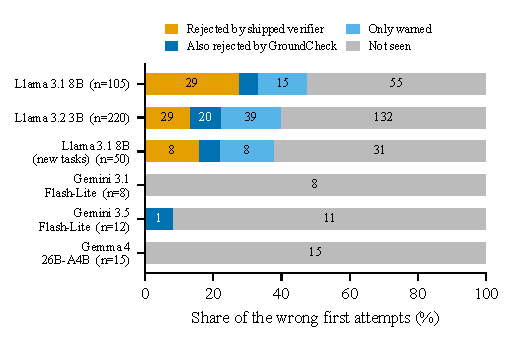
\includegraphics[width=\columnwidth]{figures/fig_e5_taxonomy}
\caption{What verification sees among the formulas each model gets wrong at attempt 1 (final system). Numbers are formulas.}
\label{fig:e5-taxonomy}
\end{figure}

\paragraph{Repair}
\begin{table*}[!t]
\caption{End-to-end execution accuracy (\%) of the production formula agent after up to two repair attempts, by repair strategy, with retrieved context. $\Delta$: percentage points over attempt 1; $p_{\text{Holm}}$: exact McNemar test against plain resampling (same tasks, paired), Holm-adjusted over the four feedback strategies of each model. Models whose first attempts are almost never rejected are omitted: no strategy has anything to repair.}
\label{tab:e5-repair}

\centering\footnotesize
\begin{tabular}{l rrr rrr rrr}
\toprule
& \multicolumn{3}{c}{\textbf{Llama~3.1 8B} (n=360)} & \multicolumn{3}{c}{\textbf{Llama~3.2 3B} (n=360)} & \multicolumn{3}{c}{\textbf{Llama~3.1 8B, new tasks} (n=180)} \\
\cmidrule(lr){2-4}\cmidrule(lr){5-7}\cmidrule(lr){8-10}
\textbf{Condition} & Acc. & $\Delta$ & $p_{\text{Holm}}$ & Acc. & $\Delta$ & $p_{\text{Holm}}$ & Acc. & $\Delta$ & $p_{\text{Holm}}$ \\
\midrule
Attempt 1 (no repair) & 70.8 & -- & -- & 38.9 & -- & -- & 72.2 & -- & -- \\
Resample (no feedback) & 71.1 & +0.3 & -- & 39.2 & +0.3 & -- & 72.8 & +0.6 & -- \\
Generic feedback & 72.2 & +1.4 & .125 & 39.7 & +0.8 & 1.000 & 72.8 & +0.6 & 1.000 \\
Shipped-verifier feedback & 74.2 & +3.3 & .007 & 39.7 & +0.8 & 1.000 & 74.4 & +2.2 & .750 \\
GroundCheck feedback & \textbf{74.4} & +3.6 & .001 & \textbf{40.0} & +1.1 & 1.000 & \textbf{75.0} & +2.8 & .375 \\
GroundCheck + suspicious & \textbf{75.3} & +4.4 & <.001 & \textbf{40.0} & +1.1 & 1.000 & \textbf{76.1} & +3.9 & .125 \\
\bottomrule
\end{tabular}
\end{table*}

Table~\ref{tab:e5-repair} and Figure~\ref{fig:e5} compare feedback strategies from the same first attempt. Asking again without feedback repairs almost nothing (\efASresample\%, $+$\efASresampleD{} points); a generic ``try again'' message gives \efASgeneric\% ($+$\efASgenericD{}); diagnostics from the shipped verifier \efASvonefb\% ($+$\efASvonefbD{}); and \gc{} diagnostics \efASvtwofb\% ($+$\efASvtwofbD{} points, 95\% interval [\efASvtwofbLo, \efASvtwofbHi]; \efASvtwofbFixed{} tasks fixed, none broken), better than resampling (Holm-adjusted $p$ \hmAHolmVtwoRes) and than the generic message ($p$ \hmAHolmVtwoGen). Also repairing on suspicious findings reaches \efASvtwofbplussusp\% ($+$\efASvtwofbplussuspD{}). The feedback of the two verifiers is not distinguishable here ($p$ \hmAHolmVtwoVone; they fix \efASvtwofbFixed{} and \efASvonefbFixed{} tasks), for the reason given above. The ordering is the same with the shipped chunk format (Table~\ref{tab:e5-repair-shipped}). Repair costs about \efAExtravtwofb{} extra model calls per task. The hosted models are absent from Table~\ref{tab:e5-repair} because they rarely give the verifier anything to reject.

\begin{figure}[t]
\centering
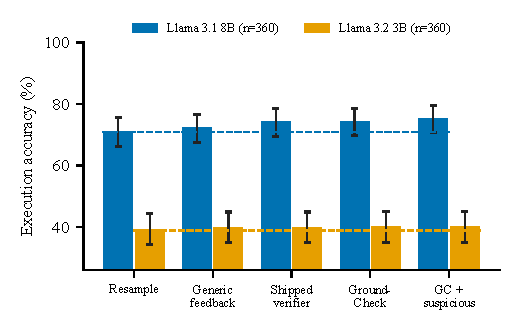
\includegraphics[width=\columnwidth]{figures/fig_e5_repair}
\caption{Execution accuracy after repair (GC: \gc) for the models whose attempts the verifier rejects often enough to compare strategies. Dashed lines: accuracy at attempt 1; error bars: 95\% Wilson intervals.}
\label{fig:e5}
\end{figure}

\paragraph{Run-to-run variation}
\ifdefined\sdASeeds
One sampled trajectory per task could mislead, so we reran the local models on the same tasks with \sdASeeds{} sampling seeds (Table~\ref{tab:e5-seeds}). Accuracy at attempt 1 with retrieved context is \sdARetr\% (SD \sdARetrSD{} points) for \efAName{} and \sdBRetr\% (SD \sdBRetrSD) for \efBName: the seed moves a model's accuracy by about a point, less than the differences between context formats or repair strategies that we interpret. For \efAName{} \gc{} feedback beats plain resampling in \sdASeedsBeat{} of \sdASeeds{} seeds, by \sdADvtwofbresample{} points on average over seeds and tasks (task-clustered 95\% interval [\sdADvtwofbresampleLo, \sdADvtwofbresampleHi]); against the shipped verifier's feedback the difference is \sdADvtwofbvonefb{} points [\sdADvtwofbvonefbLo, \sdADvtwofbvonefbHi]. For \efBName{} \gc{} feedback also beats resampling in \sdBSeedsBeat{} of \sdBSeeds{} seeds, but by only \sdBDvtwofbresample{} points [\sdBDvtwofbresampleLo, \sdBDvtwofbresampleHi]: a small effect that a single run (Table~\ref{tab:e5-repair}) cannot resolve.

\begin{table}
\caption{Run-to-run variation on the 360 main-set tasks: the same tasks rerun with 3 independent sampling seeds. The interval for the repair effect is a paired bootstrap over tasks of each task's outcome averaged over seeds.}
\label{tab:e5-seeds}

\centering\footnotesize
\begin{adjustbox}{max width=\columnwidth}\begin{tabular}{l rr}
\toprule
\textbf{Accuracy, mean (SD) over seeds} & \textbf{\shortstack[r]{Llama~3.1\\8B}} & \textbf{\shortstack[r]{Llama~3.2\\3B}} \\
\midrule
Attempt 1, active sheet only & 72.2 (0.3) & 35.8 (1.5) \\
Attempt 1, retrieved context & 71.4 (0.6) & 39.4 (0.7) \\
Resample (no feedback) & 71.6 (0.4) & 39.7 (0.7) \\
Generic feedback & 73.1 (0.8) & 40.2 (0.6) \\
Shipped-verifier feedback & 74.8 (0.7) & 40.4 (0.9) \\
GroundCheck feedback & 75.6 (1.1) & 40.8 (1.0) \\
GroundCheck + suspicious & 76.2 (0.8) & 41.0 (1.1) \\
\midrule
\gc{} feedback $-$ resample, points [95\% CI] & 4.0 [2.2, 5.9] & 1.1 [0.3, 2.2] \\
\gc{} feedback $-$ shipped feedback, points [95\% CI] & 0.7 [0.1, 1.6] & 0.5 [0.1, 1.0] \\
Seeds in which \gc{} beats resampling & 3 of 3 & 3 of 3 \\
\bottomrule
\end{tabular}\end{adjustbox}
\end{table}

\else
Further sampling seeds were not run for this version.
\fi

\paragraph{Does repair make failures safer?}
Accuracy counts whether the final cell is right and says nothing about what the wrong cells look like. Table~\ref{tab:e5-harm} accounts for every task under three policies. With \efAName, writing the first attempt unchecked leaves \hmAAsIsLoud{} cells that show an error and \hmAAsIsSilent{} that show a plausible wrong value, out of \hmAN. Withholding what \gc{} rejects, without repair, holds back \hmABlockWithheld{} formulas, all of them wrong (\hmAFalseWithheld{} correct formulas withheld), and leaves the silent errors as they were. Repairing with \gc{} feedback (Figure~\ref{fig:e5-fate}) fixes \hmAUnsafeVtwoFixed{} of the \hmAUnsafeN{} rejected attempts, but of the others \hmAUnsafeVtwo{} end as plausible wrong values and \hmAUnsafeVtwoLoud{} still show an error: the \emph{unsafe-repair rate} is \hmAUnsafeVtwoRate\% (shipped feedback: \hmAUnsafeVoneRate\%; resampling: \hmAUnsafeResRate\%, because it rarely changes anything). As a result the silent errors \emph{rise}, from \hmAAsIsSilent{} to \hmARepVtwoSilent, while the visible errors fall from \hmAAsIsLoud{} to \hmARepVtwoLoud. The picture is the same for \efBName{} (silent \hmBAsIsSilent{} to \hmBRepVtwoSilent, unsafe-repair rate \hmBUnsafeVtwoRate\%) and on the held-out tasks (\hmCAsIsSilent{} to \hmCRepVtwoSilent). \ifdefined\sdASeeds It holds across seeds: the unsafe-repair rate of \efAName{} averages \sdAUnsafevtwofb\% over the \sdASeeds{} seeds, ranging from \sdAUnsafevtwofbMin\% to \sdAUnsafevtwofbMax\%.\fi

\begin{table}
\caption{What ends up in the cell, as \% of tasks, under three policies: write the first attempt unchecked; withhold what \gc{} rejects and write the rest (no repair); repair with \gc{} feedback. \emph{Right}: evaluates to the gold value. \emph{Error}: the cell shows an error value. \emph{Silent}: a plausible but wrong value (the failure a user cannot see). \emph{Held}: nothing is written.}
\label{tab:e5-harm}

\centering\footnotesize
\begin{adjustbox}{max width=\columnwidth}\begin{tabular}{l l rrrr}
\toprule
\textbf{Model} & \textbf{Policy} & \textbf{Right} & \textbf{Error} & \textbf{Silent} & \textbf{Held} \\
\midrule
\multirow{3}{*}{Llama~3.1 8B} & Write as is & 70.8 & 18.6 & 10.6 & -- \\
 & Block rejected & 70.8 & 8.9 & 10.6 & 9.7 \\
 & Repair (\gc) & 74.4 & 12.5 & \textbf{13.1} & -- \\
\midrule
\multirow{3}{*}{Llama~3.2 3B} & Write as is & 38.9 & 30.6 & 30.6 & -- \\
 & Block rejected & 38.9 & 16.9 & 30.6 & 13.6 \\
 & Repair (\gc) & 40.0 & 24.2 & \textbf{35.8} & -- \\
\midrule
\multirow{3}{*}{Llama~3.1 8B new tasks} & Write as is & 72.2 & 16.1 & 11.7 & -- \\
 & Block rejected & 72.2 & 10.0 & 11.7 & 6.1 \\
 & Repair (\gc) & 75.0 & 12.2 & \textbf{12.8} & -- \\
\bottomrule
\end{tabular}\end{adjustbox}
\end{table}


Verification-guided repair therefore raises accuracy by turning some visible failures into correct formulas and others into invisible ones: of the visible errors it removes, only part become right. Blocking and showing the diagnostics has no such side effect, and the case for repair rests on how much a user's attention is worth. Since the outcome of a repaired formula is a valid-looking value, we regard an execution check, or showing the computed value next to the request, as the natural next step. An execution check in a scratch cell would catch the cells that show an error (\hmAAsIsLoud{} before repair and \hmARepVtwoLoud{} after, for \efAName) but none of the silent ones, which only the computed value, read against the request, can expose.

\ifdefined\exASame
\emph{Adding an execution check.} The cells that still show an error after repair are loud faults the workbook-state checks did not see. We therefore added a second stage to the pipeline, verify, repair, \emph{execute}: after \gc{} accepts a formula, it is evaluated in the workbook (in the add-on, in a scratch cell) and an error is sent back to the model (Table~\ref{tab:e5-exec}; first attempts regenerated with the same seed reproduced the stored one for \exASame{} of \exATotal{} tasks of \efAName). Of the \exALoudAfter{} cells that still show an error after \gc{} repair, the execution check fixes \exALoudFixed{}, leaves \exALoudStill{} and turns \exALoudToSilent{} into plausible wrong values; overall \exAExecCorrect{} formulas are right against \exAVtwoCorrect{} with repair alone (+\exAGained{}/$-$\exALost{} tasks, $p$ \exAP), and silent errors go from \exAVtwoSilent{} to \exAExecSilent. For \efBName{} (\exBSame{} tasks) the check fixes \exBLoudFixed{} of the \exBLoudAfter{} cells that still show an error after repair and turns \exBLoudToSilent{} into plausible wrong values; silent errors go from \exBVtwoSilent{} to \exBExecSilent. The check removes some visible errors but no silent ones: it cannot see them, and repairing an error can again produce a plausible wrong value, so the number of silent errors does not fall.

\begin{table}
\caption{What ends up in the cell (\% of tasks) when repair is followed by an execution check: after the verifier accepts a formula, the cell is evaluated and an error is sent back to the model. Only tasks whose regenerated first attempt reproduced the stored one are included, so all three policies cover the same tasks.}
\label{tab:e5-exec}

\centering\footnotesize
\begin{adjustbox}{max width=\columnwidth}\begin{tabular}{l l rrr}
\toprule
\textbf{Model} & \textbf{Policy} & \textbf{Right} & \textbf{Error} & \textbf{Silent} \\
\midrule
\multirow{3}{*}{Llama~3.1 8B} & Write as is & 75.2 & 16.2 & 8.6 \\
 & Repair (\gc) & 78.3 & 10.4 & 11.3 \\
 & Repair + execution & 80.1 & 7.6 & \textbf{12.2} \\
\midrule
\multirow{3}{*}{Llama~3.2 3B} & Write as is & 45.1 & 26.3 & 28.6 \\
 & Repair (\gc) & 46.5 & 19.2 & 34.3 \\
 & Repair + execution & 47.8 & 15.2 & \textbf{37.0} \\
\bottomrule
\end{tabular}\end{adjustbox}
\end{table}

\fi

\begin{figure}[t]
\centering
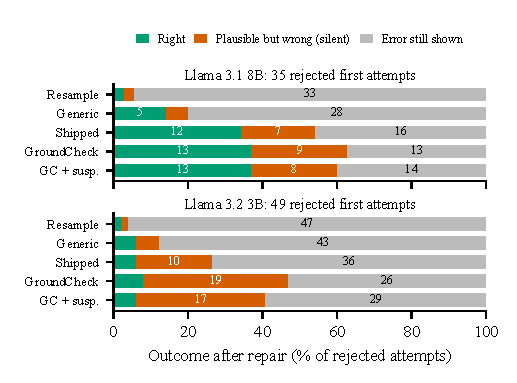
\includegraphics[width=\columnwidth]{figures/fig_e5_repair_fate}
\caption{Outcome of repair for the attempts \gc{} rejected, by strategy: right, a plausible but wrong value (silent), or an error still shown. Numbers are attempts; segments under 9\% are unlabelled.}
\label{fig:e5-fate}
\end{figure}

\paragraph{Where the models fail}
Accuracy by task template (Figure~\ref{fig:e5-templates}, Appendix~\ref{app:results}) shows the pattern behind the totals. The local models fail on the same few templates: \efATemplateZero{} of the \efNTemplates{} templates (the cross-sheet lookup) is solved on fewer than one task in twenty by \efAName{} and \efBTemplateZero{} by \efBName, whereas the hosted models' lowest template accuracies are \efDTemplateMin\%, \efETemplateMin\% and \efFTemplateMin\%. Requests that paraphrase the column names instead of quoting the headers are harder for the two local models on the main set (\efAFormS\% against \efAFormH\% for \efAName, \efBFormS\% against \efBFormH\% for \efBName) but not on the held-out set (\efCFormS\% against \efCFormH\%); we do not read more into it.
\ifdefined\efBN
\paragraph{A smaller model}
\efBName{} is correct at attempt 1 in \efBfinal\% of tasks (\efBflat\% with the active sheet only, $p$ \efBTestfinalvsflatP). It makes more of the errors that only \gc{} sees: the verifier rejects \efBCaughtTwo{} of its \efBWrong{} wrong first attempts, against \efBCaughtOne{} for the shipped one. But it makes little use of the feedback. In the main run repair raises accuracy by \efBSvtwofbD{} points ($p$ \efBSvtwofbP{} against attempt 1; \efBSvtwofbFixed{} tasks fixed), which no strategy distinguishes from resampling (Table~\ref{tab:e5-repair}); only the average over seeds resolves a gain of about a point. Feedback needs a model able to act on it. As an acceptance gate the verifier still separates the two groups: formulas it accepts are correct \efBGateAcc\% of the time and those it rejects \efBGateRej\%.
\fi
\paragraph{Hosted models}
The hosted models are right at attempt 1 on \efDfinal\%, \efEfinal\% and \efFfinal\% of their tasks (\efDflat\%, \efEflat\% and \efFflat\% with the active sheet only), so they leave the verifier almost nothing to do: they make few errors, most of them silent (\efDSilent{} of \efDWrong, \efESilent{} of \efEWrong, \efFSilent{} of \efFWrong), and no repair strategy has anything to repair. For models this accurate on these tasks the verifier is a safety net that costs nothing, and the benefit of the add-on comes from the context it supplies. This is no verdict on the value of verification for stronger models on harder work: \sheetfault{} tasks are single formulas over one or two tables, while workflow-level benchmarks find frontier agents failing far more often~\cite{zhu2026spreadsheetbench2}. The two Gemini runs were capped by the free tier's daily quota, so each covers the first tasks of a fixed hash order (\efDN{} and \efEN{} of the 360), a subset chosen without regard to difficulty; the Gemma run covers \efFN{}.
